\chapter{Panorama General}

Lo primero a considerar es la forma de comunicaci\'on entre la computadora y
la impresora, y si bien el dise\~no debe centrarse en mantener los costos de
producci\'on y construcci\'on bajos, de nada sirve un dispositivo basado en
tecnolog\'ia en desuso o pronta a desaparecer. Es por ello que en vez de
elegir m\'etodos convencionales como lo pueden ser el protocolo serial
R232\footnote{V\'ease - \url{http://es.wikipedia.org/wiki/RS-232}} o
paralelo\footnote{V\'ease - \url{http://es.wikipedia.org/wiki/Puerto_paralelo}}
(t\'ipico de impresoras antiguas), se usar\'a el protocolo serie de
comunicaci\'on \emph{USB}\footnote{El est\'andar se explica en detalle en
\fullref{cap:usb}.} \'Este est\'andar se encuentra en la mayor\'ia de los
equipos actuales y provee una versatilidad y flexibilidad como pocos.\\

Otro tema muy importante a considerar es el sistema operativo a usar en la
computadora. Si bien puede pensarse como respuesta obvia el sistema operativo
de Microsoft,
Windows\footnote{V\'ease - \url{http://www.microsoft.com/spain/windows/}} (en
su versi\'on m\'as comercializada \emph{XP}), este enfoque fuerza al potencial
usuario a comprar una licencia\footnote{Dichas licencias rondan los 100 US\$}
solo para poder utilizar la impresora.\
Entonces en vez de optar por un sistema pago se elige el sistema
operativo \emph{GNU/Linux}\footnote{V\'ease \fullref{cap:sw_libre}}
% ###--->>> Poner referencia a la secci\'on donde hablo de gnu/linux
del cual existen m\'as de mil versiones distintas, la mayor\'ia de ellas
gratuitas.
De esta forma el usuario puede obtener una copia de este sistema operativo
gratuito y usar la impresora sin mayores restricciones.\\

En la figura \ref{fig:pc_usb_printer} se muestra un esquema b\'asico de lo
dicho anteriormente. El esquema en su m\'as alto nivel ser\'a usar una
computadora con \emph{GNU/Linux} como sistema operativo y una conexi\'on
mediante \emph{USB} al dispositivo.\\

\begin{figure}[htp]
\centering
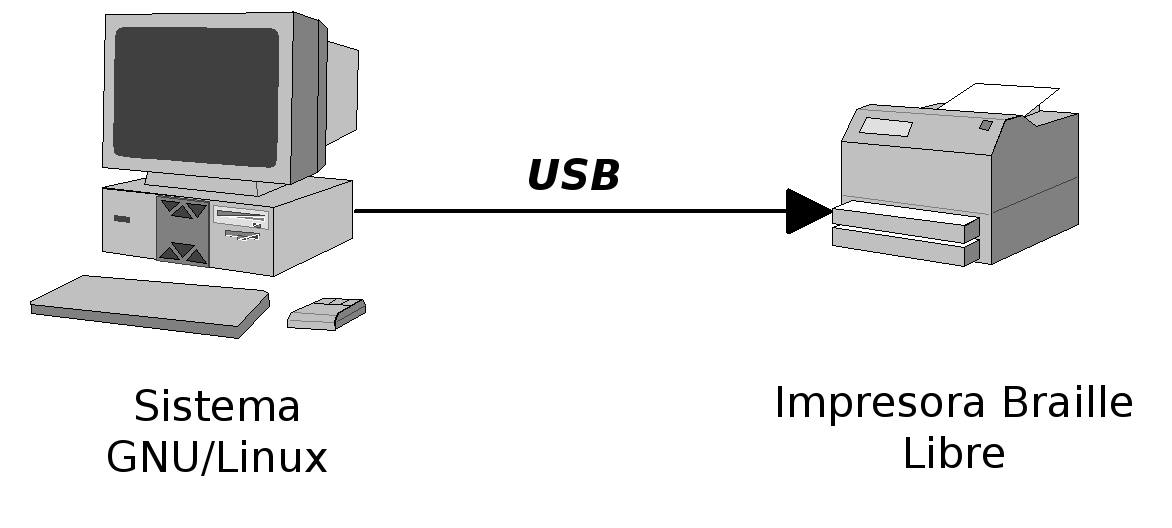
\includegraphics[width=13cm]{./img/pc_usb_printer.png}
\caption{S.O, conexi\'on e impresora}
\label{fig:pc_usb_printer}
\end{figure}

Todo el trabajo esta basado en este sencillo esquema. No obstante, y para
proveer cierta flexibilidad, cada una de las partes intervinientes es
desglosada en m\'odulos coherentes y finitos.